% Credit: TeXniCie A-eskwadraat

\documentclass[thesis]{subfiles}

\begin{document}

\newpage

\part{Structure Characterization}
\section{Theory}

In this chapter we explore a number of different ways to characterize the local `crystalline' structure in the fluid. In particular in Section \ref{subsec:rdf} we examine the radial distribution function, and in Section \ref{subsec:order} we use the local translational as well as local orientational bond order to determine local crystallinity.

\subsection{Radial Distribution Function} \label{subsec:rdf}

A simple way to look at the structure in a colloidal system is to look at the \emph{radial distribution function} $g(r)$.  The $g(r)$ can be used to get an idea of characteristic distances that appear in a system, and is often used to find the nearest neighbours, often referred to as the first neighbour shell. 

To define the radial distribution function, we start by introducing the pair correlation function 
$\rho^{(2)}(\bm r, \bm r')$,  which is the probability that there is a particle at position $\bm r$ and $\bm r'$ at the same time. Formally, the pair correlation function is defined as \cite{dijkstra2018modsim}
\begin{equation}
\rho^{(2)}(\bm r, \bm r') = \llangle \sum_i \sum_{j \neq i} \delta(\bm r - \bm r_i) \delta(\bm r' - \bm r_j) \rrangle.
\end{equation}
where $\langle \cdot \rangle$ denotes the ensemble average, $\bm r_i$ is the position of particle $i$, the sums are over all pairs of particles and $\delta$ is the Dirac delta function.
If the system is homogeneous and isotropic, then this function only depends on the distance between the particles. These simplifications lead to the radial distribution function $g(r)$ \cite{dijkstra2018modsim}
\begin{equation}
\rho^{(2)}(\bm r, \bm r') = \rho^2 g(|\bm r - \bm r'|), \label{eq:gofr}
\end{equation}
where the density $\rho$ of particles in the system has been factored out. This is done so that $g$ is dimensionless and $g(r) \rightarrow 1$ as $r \rightarrow \infty$, so long as there is no long range order (e.g. in a liquid).

Looking at Equation \ref{eq:gofr}, the radial distribution function goes to 1 in the limit of low densities. Additionally, for simple cubic crystals, like the ones formed by (slanted) cubes, we expect to see peaks in the radial distribution function at distances between simple cubic lattice sites, so at distances $a, \sqrt 2a, \sqrt 3a,\ 2a$ et cetera where $a$ is the lattice constant.

\subsection{Order Parameter} \label{subsec:order}

In this Section we will discuss the Steinhardt \emph{bond-orientational} (or simply translational) order parameter which is commonly used in the detection of crystalline order \cite{steinhardt1983bond, lechner2008accurate, van2017phase, sharma2018disorder, mickel2013shortcomings}. Aside from translational order, we also consider orientational order, because we are studying cubes which have an orientation.

\subsubsection{Translational order parameter}

First we discuss the Steinhardt order parameter in general. For a nonnegative integer $\ell$ and integers $\abs{m} \leq\ell$, we define for cube $i$ the \emph{local translational order parameter} \cite{steinhardt1983bond}
\begin{equation}
q_{\ell, m}(i) = \sum_{j} Y_{\ell, m} (\theta_{i, j}, \phi_{i, j}),
\end{equation}
where the sum is over all neighbours of cube $i$, $\theta_{i, j}$ and $\phi_{i, j}$ are the polar angle and the azimuthal angle of the vector from cube $i$'s centre to cube $j$'s centre, respectively, and $Y_{\ell, m}$ are the spherical harmonics.% given by
%\begin{equation}
%Y_{\ell, m}(\theta, \phi) = \sqrt{\frac{2\ell + 1}{4\pi}\frac{(\ell + m)!}{(\ell - m)!}}\ P_\ell^m(\cos(\theta)) \ \me^{im\phi},
%\end{equation}
%where $P_\ell^m(\cos(\theta))$ are the associated Legendre polynomials. \todo{find nice reference, define associated Legendre polynomial, maybe put this in seperate subsubsection/appendix on spherical harmonics.}

The translational correlation between neighbouring cubes $i$ and $j$ is then defined by taking the dot product and normalizing \cite{sharma2018disorder}:
\begin{equation}
d_{q_\ell}(i, j) = \frac{\sum_{m = -\ell}^\ell q_{\ell, m}(i) \cdot q^*_{\ell, m}(j)}{\sqrt{\left(\sum_{m = -\ell}^\ell \abs{q_{\ell, m}(i)}^2\right) \left(\sum_{m = -\ell}^\ell \abs{q_{\ell, m}(j)}^2\right)}}.
\end{equation}

Here the asterisk stands for complex conjugation. This translational correlation between two cubes will be a number between -1 and 1, which correspond to perfect anti-ordering and ordering respectively. Because the systems we will be studying form a simple cubic crystal, we choose to restrict our attention to the $\ell = 4$ case, as it has been observed that $q_4$ captures simple cubic order well \cite{steinhardt1983bond,mickel2013shortcomings}.

\subsubsection{Orientational order parameter} \label{subsubsec:orient order param}

For orientational order we do something similar to the translational order case, but we need to take into account the symmetries of the cube. To this end, we define three vectors for each cube: the three unit vectors perpendicular to one of the faces of the cube and each other. This definition is ambiguous, as for each face, there are two unit vectors (i.e. one pointing inward, the other pointing outward). However because we will consider only even-$\ell$ spherical harmonics, which are invariant under inversion \cite{steinhardt1983bond}, this distinction disappears.\\
For slanted cubes, there is a choice to make. The three vectors defined above could equivalently be defined as `the edges of the cube.' If we consider cubes with a slant angle smaller than 90\degr, these two definitions would differ. This difference, and an alternative definition have been studied and will be discussed in Section \ref{subsec:orientation vectors}.
\\
Just like with the translational order parameter, in general for a nonnegative integer $\ell$ and integers $ \abs{m} \leq \ell$, we define for cube $i$ the \emph{local orientational order parameter} \cite{escobedo2016effect}
\begin{equation}
i_{\ell, m}(i) = \frac{\sum_{n = 1}^3 Y_{\ell, m}(\theta_n(i), \phi_n(i))}{\sqrt{\sum_{m = -\ell}^\ell \abs{\sum_{n = 1}^3 Y_{\ell, m}(\theta_n(i), \phi_n(i))}^2}}.
\end{equation}
Here the sum over $n$ means the sum over the three axes defined above, $Y_{\ell, m}$ are again the spherical harmonics, and now $\theta_n(i)$ and $\phi_n(i)$ are the polar angle and the azimuthal angle of the vector $n$ of cube $i$, respectively.\\
Now again, we define the correlation between neighbouring cubes $i$ and $j$ by taking the dot product, where normalizing has already been done in the last step, so we define \cite{sharma2018disorder}
\begin{equation}
d_{i_\ell}(k,l) = \sum_{m = -\ell}^\ell i_{\ell, m}(k) \cdot i^*_{\ell, m}(l).
\end{equation}

Just like with the translational correlation, this will be a number between -1 and 1, corresponding to perfect anti-ordering and ordering respectively. As with the translational order case, because the systems we will be studying form a simple cubic crystal, we will restrict our attention to the $\ell = 4$ case, as we expect that orientational order will also be captured well by $i_4$.

\subsubsection{Ordered Bonds, Cubes, and Clusters}

For both types of order, having defined the order parameter for each cube as well as the order correlation between two cubes, we define a few terms which we will be using throughout this thesis.
We define a `cutoff radius,' so we say that two cubes within that cutoff radius have a \emph{bond}. If the order correlation of two bonded cubes is above an `order cutoff,' we say that two cubes have an \emph{ordered bond}. Next we define a cube to be an \emph{ordered cube} if it has at least four ordered bonds, and finally a \emph{cluster} is a collection of at least three ordered cubes which are connected in the sense that they share ordered bonds.\\

%For both the translational and orientational order, having defined the order parameter for each cube as well as the order correlation between two cubes, we continue in the same fashion for either type of order. We define a `cutoff radius,' so we call cubes within that radius \emph{bonded}. In Section \ref{subsec:res_rdf} we will determine a proper cutoff radius. Next we will define two cubes to have an \emph{ordered bond} if they are bonded and their order correlation is above a certain cutoff. In Section \ref{subsec:res_order cutoff} we will determine a proper cutoff.
%Next we define a cube to be an \emph{ordered cube} if it has at least four ordered bonds, and finally a \emph{cluster} is defined as the largest connected set of ordered cubes (with the condition that there are at least 3 cubes in the cluster), where connected means if they are bonded.

\begin{wrapfigure}{r}{0.5\textwidth}
	\vspace{-20pt}
	\centering
	\includegraphics[width=\linewidth]{images/clus1}
	\vspace{-20pt}
	\caption{A typical snapshot of a liquid of cubes, with different clusters colored differently, and all non-crystalline cubes drawn small.} \label{fig:ex.}
	\vspace{-15pt}
\end{wrapfigure}
%\vspace{-10pt}

From a visualization perspective, a nice trick to visualizing clusters is by showing particles which belong to a cluster in their true size, while showing all non-ordered cubes at only a fraction of their true size, so we can `see through' them. An example of what a fluid filled with some clusters of crystallinity might look like can be seen in Figure \ref{fig:ex.}. We will always colour different clusters in a different colour, unless there are too many different clusters.

%From a visualization perspective, a nice trick to visualizing clusters is by showing particles which belong to a cluster in their true size, while showing all non-ordered cubes at only a fraction of their true size, so we can `see through' them. An example of what a fluid filled with some clusters of crystallinity might look like can be seen in Figure \ref{fig:ex.}. We will always colour different  different clusters in a different colour, unless there are too many different clusters.
%
%\begin{figure}[H]
%	\includegraphics[width=0.3\linewidth]{images/clus1}\hfill
%	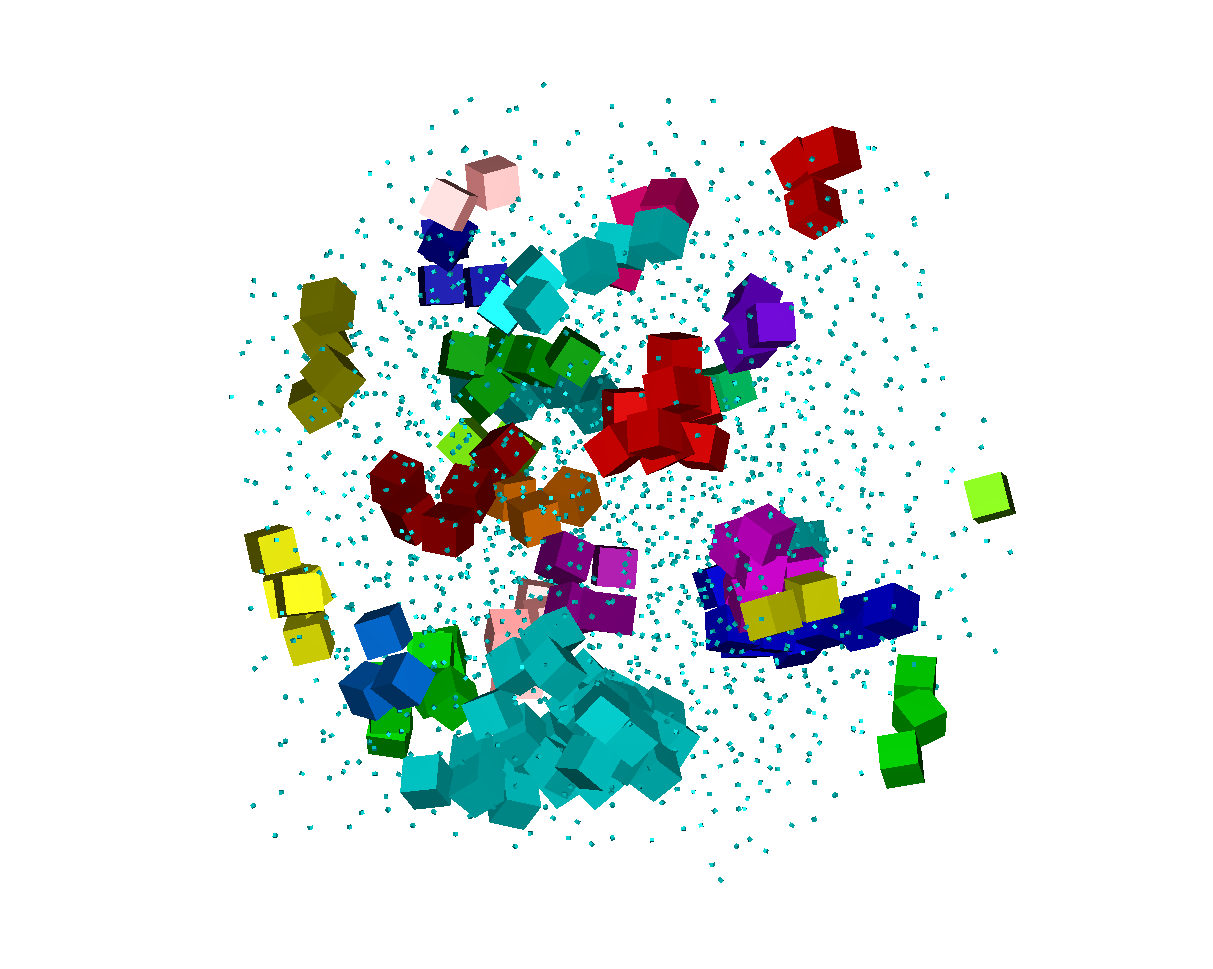
\includegraphics[width=0.3\linewidth]{images/clus2}\hfill
%	\includegraphics[width=0.3\linewidth]{images/clus3}
%	\caption{From left to right we see a system of cubes first get more clusters and finally become turn into almost one big cluster spanning the entire system.}\label{fig:ex.}
%\end{figure}


\end{document}







































